% Intended LaTeX compiler: pdflatex
\documentclass[10pt,a4paper,UTF8]{article}
\usepackage{zclorg}
\author{张朝龙}
\date{}
\title{练习:维数}
\hypersetup{
 pdfauthor={张朝龙},
 pdftitle={练习:维数},
 pdfkeywords={},
 pdfsubject={},
 pdfcreator={Emacs 25.0.50.1 (Org mode 9.0.5)}, 
 pdflang={English}}
\begin{document}

\maketitle
\tableofcontents
\titlepic{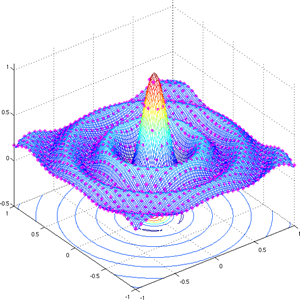
\includegraphics[scale=0.25]{../../img/sinc.PNG}}

\section{2.c.1}
\label{sec:org510ab6e}


\begin{problem}
设\(V\)是有限维的。\(U\)是\(V\)的子空间使得\(\dim U = \dim V\),证明\(U=V\)
\end{problem}

\begin{answer}
证明这类问题,我比较倾向于证明\(U\subseteq V\)并且\(V\subseteq U\)

首先证明\(U\subseteq V\),这是显然的,因为\(U\)是\(V\)的子空间,对于每一个\(u\in U\),都有\(u\in V\)。

然后证明\(V\subseteq U\). 对于每个\(v\in V\),都可以写成\(V\)的一个基的向量组合。即:\[v = \sum_{i=1}^{m} a_{i}v_{i}\]
假设\(\dim V=m\),所以\(\dim U=m\)所以\(U\)的基中向量个数为\(m\),从\(U\)的基向\(V\)的张成组的扩展是平凡的。所以\(U\)的基也构成了\(V\)的张成组。所以对于\(v\)同样也可以找到\(U\)的基的线性组合,即\[v = \sum_{i=1}^{m}b_{i}u_{i}\]

即有\(V\subseteq U\)

综上有\(U=V\)
\end{answer}
\section{2.c.2}
\label{sec:org55b9790}


\begin{problem}
证明\(\mathbf{R}^{2}\)的子空间恰为:\(\{0\},\mathbf{R}^{2}, \mathbf{R}^{2}\)中过原点的所有直线
\end{problem}

\begin{answer}
我们有\(\mathbf{R}^{2}\)子空间\(U\)的维度只能是\(0,1,2\),若\(\dim U = 0\),则\(U = \{0\}\);若\(\dim U = 2\)则有\(U = \mathbf{R}^{2}\);若\(\dim U = 1\),则有对于任何\(x\in \mathbf{R}^{2},x\neq 0\),都有:\(U=\{kx\in U:k\in \mathbf{R}\}\).
\end{answer}
\section{2.c.3}
\label{sec:org4633361}


\begin{problem}
证明\(\mathbf{R}^{3}\)的子空间恰为:\(\{0\}\),\(\{\mathbf{R}^{3}\}\),\(\{\mathbf{R}^{3}\}\)中过原点的直线,\(\{\mathbf{R}^{3}\}\)中过原点的平面。
\end{problem}

\begin{answer}
类似于2.c.2,我们有,\(\mathbf{R}^{3}\)的子空间\(U\)的维度为\(0,1,2,3\);

\begin{enumerate}
\item 若\(\dim U = 0\)则有, \(U = \{0\}\);
\item 若\(\dim U = 1\)则有, \(U = \{kx: k\in \mathbf{R}\}\);
\item 若\(\dim U = 2\)则有,\(U = \{k_1x_{1} + k_{2}x_{2}:k_{1}\in \mathbf{R},k_{2}\in \mathbf{R}\}\). 这里要求\(x_{1},x_{2}\)在\(\mathbf{R}^{3}\)中是线性独立的。
\item 若\(\dim U = 3\)则有,\(U = \mathbf{R}^{3}\)
\end{enumerate}
\end{answer}
\section{2.c.4}
\label{sec:orga38e5da}


\begin{problem}
设\(U= \{p\in \mathcal{P}_{4}(\mathbf{F}):p(6)=0\}\)求\(U\)的一个基
\end{problem}

\begin{answer}
因为\(p(6)=0\),所以一个很方便的基为\(z-6,(z-6)^{2},(z-6)^{3},(z-6)^{4}\),这个基张成空间\(U\),因此\(\dim U = 4\)。
\end{answer}

\begin{problem}
将上题求得的基扩展为\(\mathcal{P}_{4}( \mathbf{F})\)的基。
\end{problem}

\begin{answer}
因为\(\mathcal{P}_{4}( \mathbf{F})\)的维度是5,而\(\dim U = 4\),我们只需要在扩展一维即可,一个简单的扩展是\(a:a\in \mathbf{F}\)
\end{answer}

\begin{problem}
求\(\mathcal{P}_{4}( \mathbf{F})\)的一个子空间\(W\)使得\(\mathcal{P}_{4}( \mathbf{F}) = U\oplus W\)
\end{problem}

\begin{answer}
由第二步得知:\(W=\{a:a\in \mathbf{F}\}\),\(\mathcal{P}_{4}( \mathbf{F}) = U \oplus W\)
\end{answer}

\section{2.c.5}
\label{sec:org043dafc}


\begin{problem}
设\(U = \{p\in \mathcal{P}_{4}(R):p^{''}(6)=0\}\)求\(U\)的一个基
\end{problem}

\begin{answer}
一个简单的基为\(1,z-6,(z-6)^{2},(z-6)^{3},(z-6)^{4}\)
\end{answer}

\begin{problem}
将第一步求得的基扩充为\(\mathcal{P}_{4}(\mathbf{R})\)的基
\end{problem}

\begin{answer}
因为\(\dim U = 4\),\(\dim \mathcal{P}_{4}(\mathbf{F}) = 5\),所以\(U = \mathcal{P}_{4}(\mathbf{F})\).所以从\(U\)的基向\(\mathcal{P}_{4}(\mathbf{F})\)的基扩展是平凡的。即\(U\)的基就是\(\mathcal{P}_{4}(\mathbf{F})\)的基
\end{answer}

\begin{problem}
求\(\mathcal{P}_{4}(\mathbf{R})\)的一个子空间\(W\)使得\(\mathcal{P}_{4}( \mathbf{R}) = U\oplus W\)
\end{problem}

\begin{answer}
由第二步得\(\dim W = 0\),即\(W = \{0\}\)
\end{answer}

\section{2.c.6}
\label{sec:org82c02df}


\begin{problem}
设\(U=\{p\in \mathcal{P}_{4}( \mathbf{F}):p(2)=p(5)\}\) 求\(U\)的一个基
\end{problem}

\begin{answer}
对于\(f(x) = ax^{4} + bx^{3} + cx^{2} + dx +e\),利用\(f(2) = f(5)\),我们得到一个关于\(a,b,c,d,e\)的线性方程组。这个线性方程组的解的维度是\(4\),也就是说\(f(x)\)的系数只需要使用\(4\)个实数即可表示。所以\(U\)的维度是4.

\(U\)的一个简单的基是\(1, (x-2)(x-5), x(x-2)(x-5),x^{2}(x-2)(x-5)\)
\end{answer}


\begin{problem}
扩展\(U\)的基,得到\(\mathcal{P}_{4}( \mathbf{F})\) 的一个基。
\end{problem}

\begin{answer}
从上题可得,可以从\(1, (x-2)(x-5), x(x-2)(x-5),x^{2}(x-2)(x-5)\)扩展为\(1,x,(x-2)(x-5), x(x-2)(x-5),x^{2}(x-2)(x-5)\)
\end{answer}

\begin{problem}
求\(\mathcal{P}_{4}(\mathbf{F})\)的一个子空间\(W\)使得\(\mathcal{P}_{4}( \mathbf{F}) = U\oplus W\)
\end{problem}

\begin{answer}
\(W = \{cx:c\in \mathbf{F}\}\)
\end{answer}
\section{2.c.7}
\label{sec:orga14319e}


\begin{problem}
设\(U=\{p\in \mathcal{P}_{4}( \mathbf{F}):p(2)=p(5)=p(6)\}\) 求\(U\)的一个基.
\end{problem}

\begin{answer}
根据2.c.6,可以得一个基\(1,(x-2)(x-5)(x-6),x(x-2)(x-5)(x-6)\)
\end{answer}


\begin{problem}
扩展\(U\)的基,得到\(\mathcal{P}_{4}( \mathbf{F})\) 的一个基。
\end{problem}

\begin{answer}
可以从\(1,(x-2)(x-5)(x-6),x(x-2)(x-5)(x-6)\),扩展到\(1,x,x^{2},(x-2)(x-5)(x-6),x(x-2)(x-5)(x-6)\)
\end{answer}

\begin{problem}
求\(\mathcal{P}_{4}(\mathbf{F})\)的一个子空间\(W\)使得\(\mathcal{P}_{4}( \mathbf{F}) = U\oplus W\)
\end{problem}

\begin{answer}
\(W = \{c_{1}x + c_{2}x^{2}:c_{1}\in \mathbf{F},c_{2} \in \mathbf{F}\}\)
\end{answer}

\section{2.c.8}
\label{sec:org32a49e5}


\begin{problem}
设\(U=\{p\in \mathcal{P}_{4}(\mathbf{R}):\int_{-1}^{1}p = 0\}\),求\(u\)的一个基
\end{problem}

\begin{answer}
对于多项式\(f(x) = ax^{4} + bx^{3} + cx^{2} + dx + e\),考虑\(\int_{-1}^{1}f = 0\),我们得到
\begin{equation}
\label{eq:1}
\frac{a}{5} + \frac{d}{3} + e = 0
\end{equation}
这个关于\(a,b,c,d,e\)的线性方程组的解空间有:
\begin{eqnarray}
\label{eq:2}
&&(0,1,0,0,0) \\
&&(\frac{-5}{3},0,1,0,0) \\
&&(0,0,0,1,0) \\
&&(-5,0,0,0,1) 
\end{eqnarray}
因为所有系数满足以上解的组合的线性方程组的系数确定的多项式都满足\(\int_{-1}^{1}f = 0\),并且并且以上给出的四个解释线性无关的(可以根据线性无关组定义证明)。所以把四个解带入\(f(x)\)我们得到了一个\(U\)的基\(x^{3},\frac{-5}{3}x^{4} +x^{2}, x, -5x^{4} + 1\)。

对于这个基我们还可以做一些线性组合比如\((3)(\frac{-5}{3}x^{4} +x^{2}) + (-1)(-5x^{4} + 1) = 3x^{2} -1\)

显然所以这个基可以变为:\(x^{3},3x^{2} -1, x, -5x^{4} + 1\)。
\end{answer}

\begin{problem}
扩展\(U\)的一个基,得到\(\mathcal{P}_{4}( \mathbf{R})\)的一个基。
\end{problem}

\begin{answer}
扩展\(x^{3},3x^{2} -1, x, -5x^{4} + 1\)到\(1, x^{3},3x^{2} -1, x, -5x^{4} + 1\)。
\end{answer}

\begin{problem}
求\(\mathcal{P}_{4}(\mathbf{R})\)的一个子空间\(W\)使得\(\mathcal{P}_{4}( \mathbf{R}) = U\oplus W\)
\end{problem}

\begin{answer}
从前文得知,\(W = \{c:c\in \mathbf{R}\}\),所以有\(\mathcal{P}_{4}( \mathbf{R}) = U\oplus W\)
\end{answer}
\section{2.c.9}
\label{sec:org0ff89ad}


\begin{problem}
设\(v_{1},v_{2},\ldots ,v_{m}\)在\(V\)中是线性无关的,并设\(w\in V\),证明:\(\dim span(v_{1} + w,\ldots ,v_{m}+w) \geq m-1\)
\end{problem}

\begin{answer}
在这个题目中出现了不等式,我们知道一个线性空间中线性无关组的中向量的个数小于等于张成空间向量组的个数。我们来构建一个维数为\(m-1\)的线性无关组。

考虑\(v_{2} -v_{1} = (v_{2} + w) - (v_{1} + w)\),所以\(v_{2}-v_{1}\in span(v_{1} + w,\ldots ,v_{m}+w)\),同理对于\(v_{i} - v_{1},2\leq i \leq m\)都有\(v_{i}-v_{1}\in span(v_{1} + w,\ldots ,v_{m}+w)\). 

接下来证明\(v_{i}-v_{1}, 2\leq i \leq m\)是线性无关的。假设:
\begin{equation}
\label{eq:4}
a_{1}(v_{2} - v_{1}) + \ldots a_{m-1}(v_{m} - v_{1}) = 0
\end{equation}
则有
\begin{equation}
\label{eq:5}
(-a_{1} - a_{2} - \ldots -a_{m-1})v_{1} + a_{1}v_{2} + \ldots a_{m-1} v_{m} = 0
\end{equation}

因为\(v_{1},\ldots ,v_{m}\)是线性无关的,则有\(a_{i} = 0, 1\leq i \leq m\)
\end{answer}

\section{2.c.10}
\label{sec:org1a28de9}


\begin{problem}
假设\(p_{0},\ldots ,p_{m}\in \mathcal{P}( \mathbf{F})\)使得每个\(p_{j}\)的次数为\(j\),证明\(p_{0},p_{1},\ldots ,p_{m}\)是\(\mathcal{P}( \mathbf{F})\)的基
\end{problem}

\begin{answer}
由于每个\(p_{j}\)的次数为\(j\),则有:
\begin{equation}
\label{eq:6}
0 = a_{0}p_{0} + \ldots a_{m}p_{m}
\end{equation}
时只有,\(a_{j},0\leq j \leq m,j\in \mathbf{Z}\)满足要求,因此\(p_{0},\ldots ,p_{m}\)是线性无关的,又因为这个线性无关组的向量个数是\(m+1\)和\(\mathcal{P}_{m}(\mathbf{F})\)的维度相同,所以\(p_{0},\ldots ,p_{m}\)是\(\mathcal{P}_{m}(\mathbf{F})\)的基。
\end{answer}
\section{2.c.11}
\label{sec:org9aee178}


\begin{problem}
设\(U\)和\(W\)是\(\mathbf{R}^{8}\)的子空间使得有\(\dim U = 3,\dim W = 5\),\(U+W = \mathbf{R}^{8}\),证明\(\mathbf{R}^{8} = U\oplus W\)
\end{problem}

\begin{answer}
首先假设\(u_{1},u_{2},u_{3}\)是\(U\)的基,所以\(u_{1},u_{2},u_{3}\)是\(V\)的线性无关组,我们可以把\(u_{1},u_{2},u_{3}\)扩充成\(V\)的一组基,又因为\(\dim V  =8\),所以只用扩充\(5\)个线性无关向量\(w_{1},w_{2},w_{3},w_{4},w_{5}\)即可。

假设这\(5\)个线性无关向量全都来自于\(W\),这是可能的因为\(\dim W = 5\)。接下来我们证明\(U\cap W = \{0\}\)

\begin{equation}
\label{eq:8}
\dim U\cap W = \dim U + \dim W - \dim (U+W)
\end{equation}

因为\(U+W = \mathbf{R}^{8}\),则有\(\dim U\cap W = 0\).

因为\(U+W=\mathbf{R}^{8}\),且\(\dim U\cap W = 0\),所以\(U\oplus W=\mathbf{R}^{8}\).
\end{answer}
\section{2.c.12}
\label{sec:orgee1c804}


\begin{problem}
设\(U,W\)均为\(\mathbf{R}^{9}\)的\(5\)维子空间,则有\(U\cap W \neq \{0\}\)
\end{problem}

\begin{answer}
同2.c.11一样,这里也用到空间维数定理。

\begin{equation}
\label{eq:9}
\dim(U_{1}\cap U_{2} = \dim U_{1} + \dim U_{2} - \dim (U_{1}+U_{2})
\end{equation}
因为\(\dim (U_{1} + U_{2}) \leq dim \mathbf{R}^{9}\),所以:
\begin{equation}
\label{eq:10}
\dim(U_{1}\cap U_{2} \geq \dim U_{1} + \dim U_{2} - \dim \mathbf{R}^{9} \geq 1
\end{equation}

所以\(U_{1}\cap U_{2} \neq \{0\}\)
\end{answer}
\section{2.c.13}
\label{sec:orga3d65d3}

\begin{problem}
设\(U\)和\(W\) 均为\(\mathbf{R}^{4}\)中的\(4\)维子空间,证明在\(U\cap W\)中存在两个向量使得其中任何一个都不是另外一个的标量倍。
\end{problem}

\begin{answer}
这个题目2.c.11,2.c.12的变形,必须有:
\begin{equation}
\label{eq:11}
\dim(U\cap W \geq \dim U + \dim W - \dim \mathbf{R}^{6} \geq 2
\end{equation}

因为\(\dim(U\cap W \geq 2\),则必有\(U\cap W\)中至少有两个向量线性无关,根据线性无关的定义这两个向量的其中任何一个都不是另外一个的标量倍,不然就会产生矛盾。

比如\(u_{1},u_{2}\)是属于\(U\cap W\)的两个线性无关的向量,如果\(u_{1} = \lambda u_{2}\),则有\(u_{1} - \lambda u_{2} =0\),这与线性无关组要求的\(0\)的唯一表示方法矛盾。
\end{answer}

\section{2.c.14}
\label{sec:org984cf93}


\begin{problem}
设\(U_{1},\ldots ,U_{m}\)均为\(V\)的有限维子空间。证明\(U_{1} + \ldots + U_{m}\)是有限维的且
\begin{equation}
\label{eq:12}
\dim ( U_{1} + \ldots + U_{m}) \leq \dim U_{1} + \ldots + \dim U_{m}
\end{equation}
\end{problem}

\begin{answer}
首先子空间的和是包含这些子空间的最小子空间,所以\(U_{1}+\ldots +U_{m}\)是\(V\)中包含\(U_{i}\)的最小子空间。所以有\(\dim(U_{1} + \ldots + U_{m}) \leq \dim V\)。所以\(U_{1}+\ldots +U_{m}\)是有限维的。

另外有,取\(\mathcal{U}_{i}\)为\(U_{i}\)的基,我们知道\(span( \mathcal{U}_{1},\ldots , \mathcal{U}_{m})\)张成了\(U_{1}+U_{2}+\ldots +U_{m}\),而\(\mathcal{U}_{1},\ldots , \mathcal{U}_{m}\)可以简化为\(U_{1}+\ldots +U_{m}\)的一组基。这组基中的向量个数不会超过\(\mathcal{U}_{1},\ldots , \mathcal{U}_{m}\)中向量个数之和。

即:
\begin{equation}
\label{eq:13}
\dim(U_{1} + \ldots U_{m}) \leq \dim U_{1} + \ldots + \dim U_{m}
\end{equation}
\end{answer}
\section{2.c.15}
\label{sec:org7be125f}


\begin{problem}
设\(V\)是有限维的且\(\dim V=n\geq 1\),证明存在\(V\)的\(1\)维子空间\(U_{1},\ldots ,U_{n}\)使得:
\begin{equation}
\label{eq:15}
V=U_{1}\oplus \ldots \oplus U_{n}
\end{equation}
\end{problem}

\begin{answer}
因为\(\dim V = n\),所以可以找到\(n\)个线性无关向量构成\(V\)的基。这\(n\)个线性无关向量 用\(v_{1},\ldots ,v_{n}\)表示。基中的每个向量都可以张成一个\(V\)的子空间,如此张成了\(n\)个子空间\(U_{i},i\in \{1,\ldots ,n\}\) 

对于\(V\)总的任意向量\(v\),都可以表示成
\begin{equation}
\label{eq:16}
v= a_{1}v_{1} + \ldots + a_{n}v_{n}
\end{equation}

因此\(V = U_{1}+ \ldots +U_{n}\),由于\(v_{i},i\in \{1,\ldots ,n\}\) 则这个表示是唯一的。根据直和的定义有:
\begin{equation}
\label{eq:17}
V = U_{1}\oplus \ldots \oplus U_{n}
\end{equation}
\end{answer}
\section{2.c.16}
\label{sec:org7131aaf}


\begin{problem}
设\(U_{1},\ldots ,U_{m}\)均为\(V\)的有限维子空间,使得\(U_{1}+ \ldots +U_{m}\)是直和,证明\(U_{1} \oplus \ldots \oplus U_{m}\)是有限维的且:
\begin{equation}
\label{eq:18}
\dim U_{1}\oplus + \ldots + U_{m} = \dim U_{1} + \ldots + \dim U_{m}
\end{equation}
\end{problem}

\begin{answer}
这个题目是2.c.14的翻版。

首先子空间的和是包含这些子空间的最小子空间,所以\(U_{1}\oplus \ldots \oplus U_{m}\)是\(V\)中包含\(U_{i}\)的最小子空间。所以有\(\dim(U_{1} + \ldots + U_{m}) \leq \dim V\)。所以\(U_{1}\oplus \ldots \oplus U_{m}\)是有限维的。

另外有,取\(\mathcal{U}_{i}\)为\(U_{i}\)的基,我们知道\(span( \mathcal{U}_{1},\ldots , \mathcal{U}_{m})\)张成了\(U_{1}\oplus U_{2}\oplus \ldots \oplus U_{m}\),而\(\mathcal{U}_{1},\ldots , \mathcal{U}_{m}\)可以简化为\(U_{1}+\ldots +U_{m}\)的一组基。这个张成组可以简化为\(U_{1}\oplus U_{2}\oplus \ldots \oplus U_{m}\)的一个基,但是在简化过程中,我们会发现,这个简化是平凡的,根据直和的定义,我们不能从这些向量中去掉任何一个向量。基中的向量个数等于\(\mathcal{U}_{1},\ldots , \mathcal{U}_{m}\)中向量个数之和。

即:
\begin{equation}
\label{eq:20}
\dim(U_{1} \oplus \ldots \oplus U_{m}) = \dim U_{1} + \ldots + \dim U_{m}
\end{equation}
\end{answer}
\section{2.c.17}
\label{sec:org4c266fe}


\begin{problem}
通过与有限集合中三个子集之并的元素公式相类比,我们可能猜测,如果\(U_{1},U_{2},U_{3}\)是有限维向量空间的子空间,那么:
\begin{eqnarray}
\label{eq:19}
\dim (U_{1} + U_{2} + U_{3})&=& \dim U_{1} + \dim U_{2} + \dim U_{3} \\
&& - \dim(U_{1}\cap U_{2}) - \dim(U_{1}\cap U_{3}) - \dim(U_{2}\cap U_{3}) \\
&& + \dim(U_{1}\cap U_{2} \cap U_{3})
\end{eqnarray}
\end{problem}


\begin{answer}
这个题目放在空间的概念里忽略了一个问题:

一个\(n\)维的空间可以有大于\(n\)个子空间并且这些子空间互不相交。
\end{answer}
\end{document}
